\section{Kompaktní množiny a konvergence}\label{sec:konvergence-hmp}

\begin{theorem}\label{thm:konvergence-hmp}
    Nechť $A_1,A_2,\ldots$ je nerostoucí posloupnost množin,~kde $A_i\in\hyperspace(X)$ pro každé $i\in\N$. Pak posloupnost $A_1,A_2,\ldots$ konverguje k~množině
    \[A=\bigcap_{i=1}^\infty A_i\]
    v~Hausdorffově metrice.
\end{theorem}
\begin{proof}
    Nechť je dáno $\varepsilon>0$. Zjevně pro každé $i$ je $A\subseteq A_i$,~tzn. $A\subseteq(A_i)_\varepsilon$.
    
    Nyní ukážeme,~že $\hausdorffmetric(A,A_i)<\varepsilon$ pro každé $i\geqslant i_0$. Systém
    \[\mathcal{F}=\set{(A_i)_\varepsilon}\cup\set{X\setminus A_i\mid i\in\N}\]
    tvoří otevřené pokrytí množiny $A_1$ pro každé $i\in\N$. Podle předpokladu je však $A_1$ kompaktní,~tedy z~$\mathcal{F}$ lze vybrat konečné podpokrytí. Specificky existuje $i_0\in\N$,~takové,~že pro všechna $i\geqslant i_0$ je systém
    \[\mathcal{G}=\set{X\setminus A_i}\cup\set{(A)_\varepsilon}\]
    pokrytím $A_1$ a $\mathcal{G}\subseteq\mathcal{F}$ (viz obrázek \ref{fig:konvergence-hmp}). Z~toho plyne,~že $A_i\subseteq (A)_\varepsilon$ a tedy $\hausdorffmetric(A,A_i)<\varepsilon$.
\end{proof}
\begin{figure}[h]
    \centering
    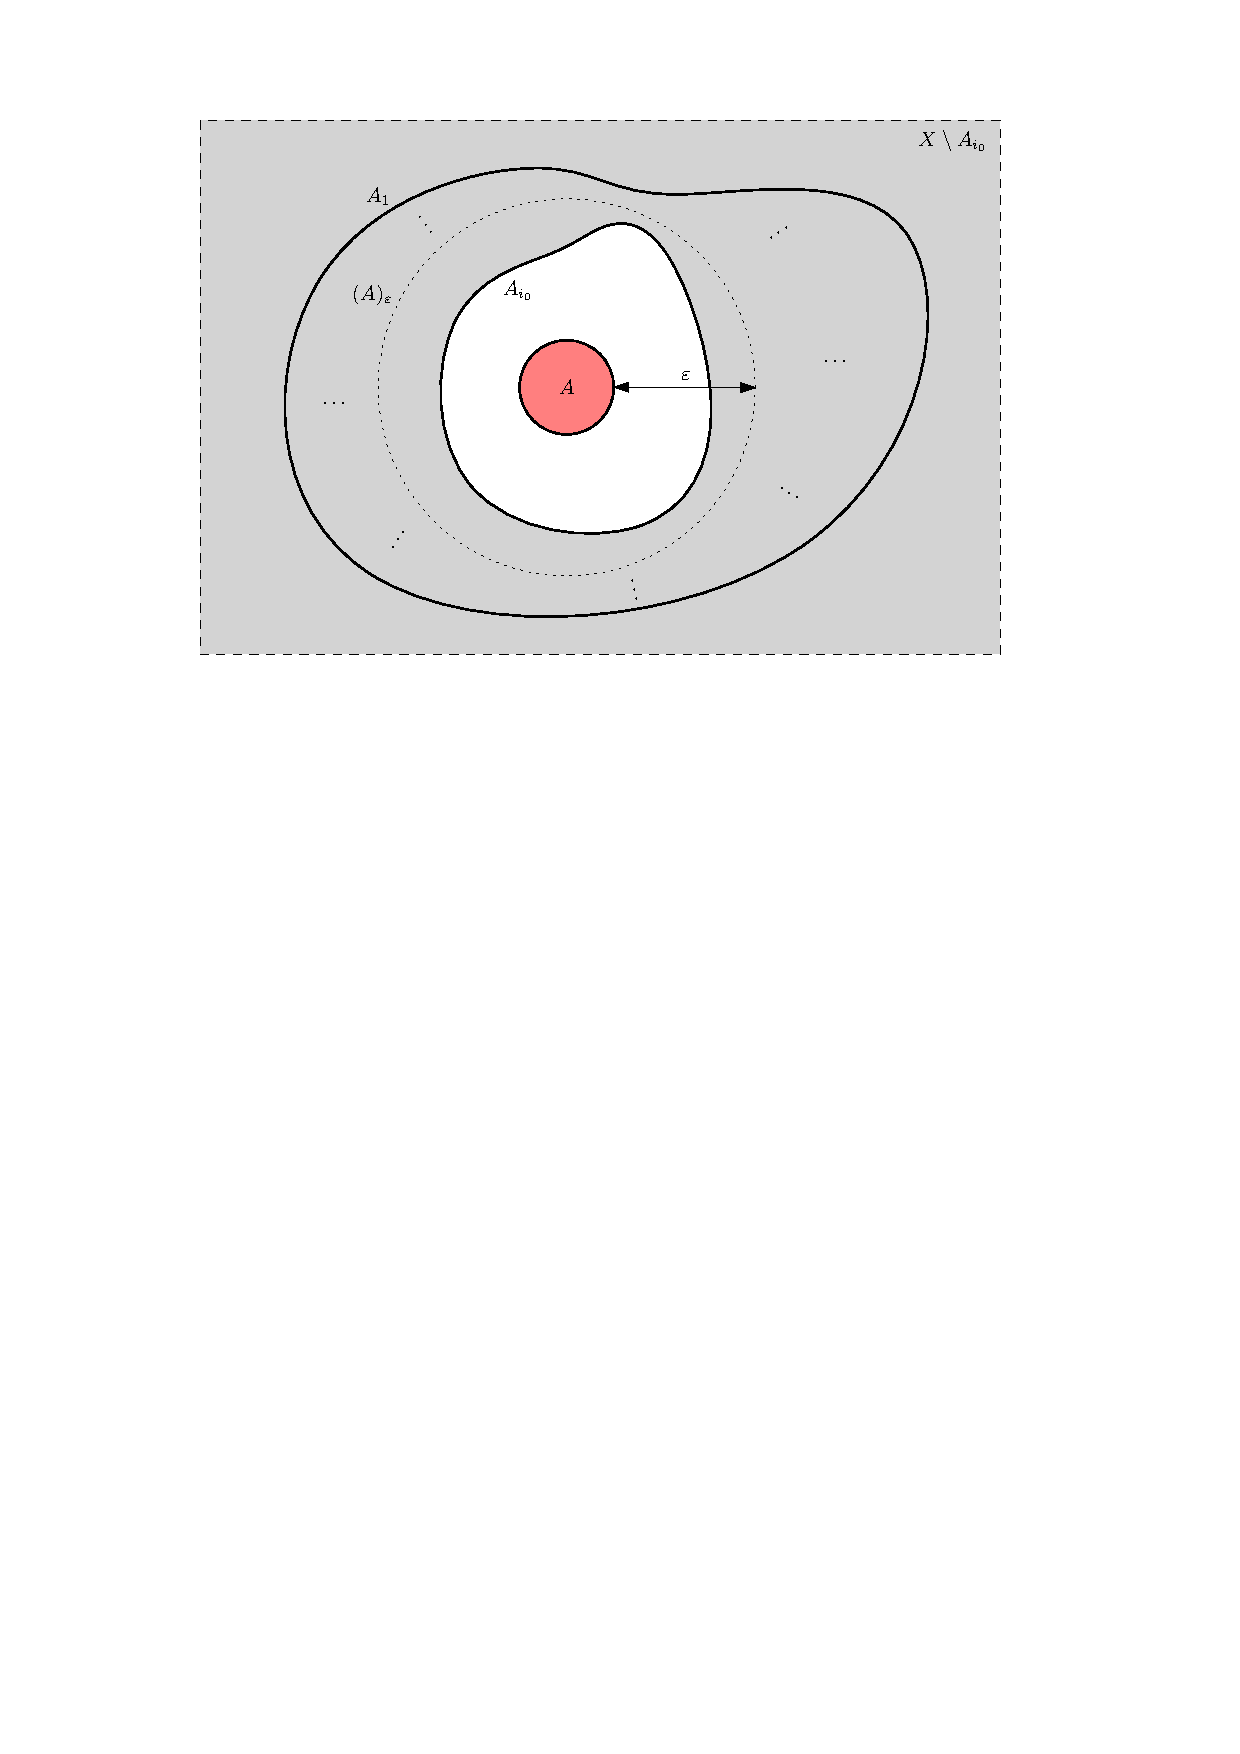
\includegraphics{ch03-ilustrace-vety-o-konvergenci.pdf}
    \caption{Ilustrace věty \ref{thm:konvergence-hmp}}
    \label{fig:konvergence-hmp}
\end{figure}

V souvislosti s~konvergencí v~prostoru $(\hyperspace(X),\hausdorffmetric)$ nebude na škodu si připomenout jedno známé související tvrzení z~matematické analýzy.
\begin{theorem}[Cantorova\index{Cantorova věta}]\label{thm:cantor}
    Následující tvrzení jsou ekvivalentní:
    \begin{enumerate}[label=(\roman*)]
        \item\label{thm:cantor-uplnost} $(X,\varrho)$ je úplný metrický prostor.
        \item\label{thm:cantor-nekl-posl-mnozin} Je-li $A_1,A_2,\ldots$ neklesající posloupnost uzavřených množin,~kde $A_i\subseteq X$ pro každé $i\in\N$,~takových,~že $\diam{A_i}\to 0$,~pak existuje $x\in X$ splňující
        \[\bigcap_{i=1}^\infty A_i=\set{x}.\]
    \end{enumerate}
\end{theorem}
Věta \ref{thm:cantor} je v~podstatě rozšířením Cantorova principu vnořených intervalů v~$\R$. Speciálně z~toho vyplývá,~že i~v Hausdorffově metrickém prostoru platí podmínka \ref{thm:cantor-nekl-posl-mnozin},~neboť z~věty \ref{thm:uplnost-hmp} víme,~že $(\hyperspace(X),\hausdorffmetric)$ tvoří úplný metrický prostor.

\begin{theorem}\label{thm:stejnometrna-konvergence-hmp}
    Nechť $(X,\varrho_1),(Y,\varrho_2)$ jsou metrické prostory a zobrazení $\set{f_i}_{i=1}^\infty$,~kde $\mapping{f_i}{X}{Y}$ pro každé $i\in\N$,~tvoří posloupnost funkcí stejnoměrně konvergující\index{stejnoměrná konvergence} k~$f$. Pak posloupnost $f_1(X),f_2(X),\ldots$ konverguje k~$f(X)$ na metrickém prostoru $(\hyperspace(Y),\hausdorffmetric)$. (Převzato z~\citep[str. 74]{Edgar2008})
\end{theorem}
\begin{proof}
    Mějme $\varepsilon>0$. Ukážeme,~že $\hausdorffmetric(f(X),f_i(X))<\varepsilon$ pro $i\geqslant i_0$. Funkce $f_1,f_2,\ldots$ konvergují k~$f$ stejnoměrně,~tzn.
    \[\forall\varepsilon>0\;\exists i_0\in\N\;\forall i\geqslant i_0\;\forall x\in X:\varrho_2(f(x),f_i(x))<\varepsilon.\]
    Tzn.~pro každé $x\in X$ a $i\geqslant i_0$ platí
    \[\varrho_2(f(x),f_i(X))\leqslant\varrho_2(f(x),f_i(x))<\varepsilon.\]
    a též
    \[\varrho_2(f_i(x),f(X))\leqslant\varrho_2(f_i(x),f(x))=\varrho_2(f(x),f_i(x))<\varepsilon.\]
    Z~toho vyplývá,~že
    \[f(X)\subseteq (f_i(X))_\varepsilon\;\text{a zároveň}\;f_i(X)\subseteq (f(X))_\varepsilon\]
    neboli $\hausdorffmetric(f(X),f_i(X))<\varepsilon$.
\end{proof}
\begin{remark}
    Předpoklad stejnoměrné konvergence ve větě \ref{thm:stejnometrna-konvergence-hmp} je důležitý. Mějme např. metrický prostor $X=\langle0,1\rangle$ se standardní eukleidovskou metrikou a definujme posloupnost funkcí
    \[\mapping{f_n}{\langle0,1\rangle}{\R},\;f_n(x)=x^n.\]
    Limitou je funkce $f$,~přičemž
    \[f(x) = \begin{cases}
        0 & x \in \langle0,1),\\
        1 & x = 1.
        \end{cases}\]
    Posloupnost konverguje k~funkci $f$ pouze bodově,~nikoliv stejnoměrně. Pro celý interval je $f(X)=\set{0,1}$,~nicméně
    \[\hausdorffmetric(\langle0,1\rangle,\set{0,1})=\dfrac{1}{2}.\]
    Tedy neplatí,~že $f_n(X)\rightrightarrows f(X)$ v~$(\hyperspace(\R),\hausdorffmetric)$.
\end{remark}